\documentclass{beamer}
\usepackage[utf8]{inputenc}
\usepackage[russian]{babel}
\usepackage{graphicx}
\usepackage{amsmath, amssymb}
\usepackage{booktabs}
\usepackage{multicol}
\usepackage{animate} 

\title{Lab 207: Сжатие тензорного представления синтетического видео с помощью HOSVD}
\author{Ребриков Алексей, Б05-105}
\date{\today}

\begin{document}

\frame{\titlepage}

\begin{frame}{Цель лабораторной работы}
\begin{itemize}
  \item Применение метода HOSVD для снижения размерности видеоданных
  \item Визуализация синтетического видео в 3D
  \item Анализ потерь качества при сжатии по разным осям
\end{itemize}
\end{frame}

\begin{frame}{Описание данных}
\begin{itemize}
  \item Синтетическое видео: вращающаяся пирамида
  \item Размерность тензора: $64 \times 64 \times 3 \times 3 \times 4 \times 20$
  \item Измерения: ширина, высота, цвет, азимут, высота камеры, время
\end{itemize}
\end{frame}

\begin{frame}{Метод HOSVD}
\begin{itemize}
  \item Разложение тензора $\mathcal{X} \in \mathbb{R}^{n_1 \times n_2 \times \dots \times n_d}$:
  \begin{equation*}
    \mathcal{X} = \mathcal{S} \times_1 U^{(1)} \times_2 U^{(2)} \dots \times_d U^{(d)}
  \end{equation*}
  \item $U^{(k)}$ — ортонормированные матрицы сингулярных векторов (SVD по оси $k$)
  \item $\mathcal{S}$ — ядро (core tensor), несёт основную информацию
\end{itemize}
\end{frame}

\begin{frame}{Сжатие: идея}
\begin{itemize}
  \item Сокращаем число компонент $r_k < n_k$ по каждой оси
  \item Уменьшается объём данных, сохраняется структура
  \item Исследуем влияние сжатия по разным осям на качество восстановления
\end{itemize}
\end{frame}

\begin{frame}{Оригинальное видео (до сжатия)}
    \centering
    \animategraphics[loop,controls,width=0.9\linewidth]{10}{original_frames/orig_}{000}{019}
\end{frame}

\begin{frame}{Сжатое видео после HOSVD}
    \centering
    \animategraphics[loop,controls,width=0.9\linewidth]{10}{reduced_frames/reduced_}{000}{019}
\end{frame}
    
    

\begin{frame}{Метрики качества}
\begin{itemize}
  \item PSNR — отношение сигнала к шуму (в децибелах)
  \item SSIM — структурное сходство
  \item Оценка проводится по всем кадрам на разных уровнях сжатия, усредняется, считается ошибка (выборочная дисперсия)
\end{itemize}
\end{frame}

\begin{frame}{PSNR при разных стратегиях сжатия}
\centering
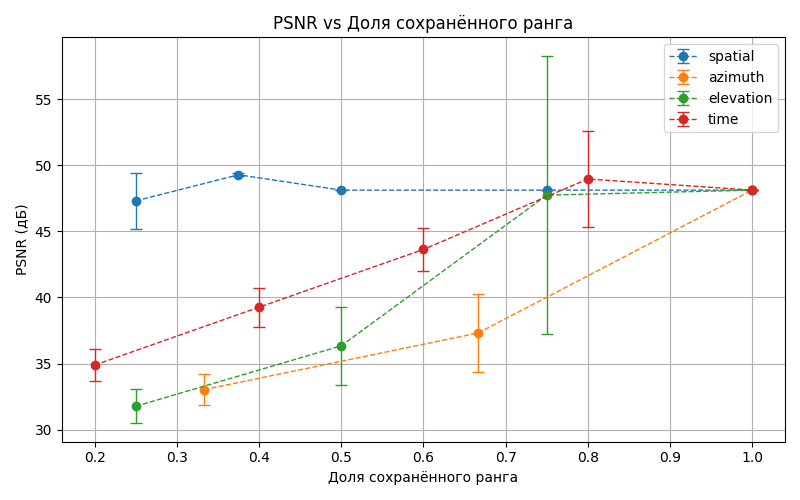
\includegraphics[width=0.95\textwidth]{psnr_all.png}
\end{frame}

\begin{frame}{SSIM при разных стратегиях сжатия}
\centering
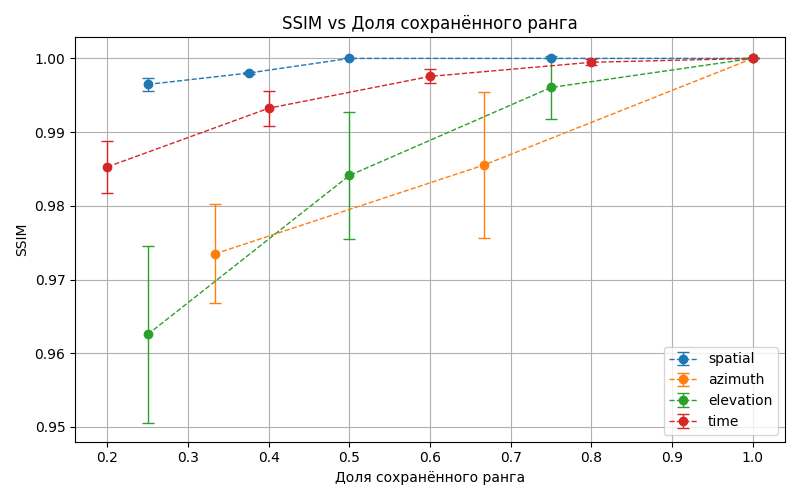
\includegraphics[width=0.95\textwidth]{ssim_all.png}
\end{frame}

\begin{frame}{Выводы}
\begin{itemize}
  \item Сжатие пространственных координат вносит наименьшие искажения
  \item Хуже всего сохраняется качество при сжатии углов обзора
  \item По разным метрикам меняется порядок <<типов>> сжатия
\end{itemize}
\end{frame}

\end{document}
